\documentclass[12pt]{report}
\usepackage[utf8]{inputenc}
\usepackage[margin=1in]{geometry}
\usepackage{graphicx}
\usepackage{float}
\usepackage{amsmath}
\usepackage{hyperref}

\title{Comprehensive Service Request Performance Analysis}
\author{Data Analysis Team}
\date{\today}

\begin{document}

\maketitle
\tableofcontents

\chapter{Acknowledgment Time Analysis}

\section{Statistical Overview}
The analysis of service request acknowledgment times reveals a complex distribution pattern with the following key statistics:
\begin{itemize}
    \item Median: 688.0 minutes (11.47 hours)
    \item Mean: 2,890.31 minutes (48.17 hours)
    \item Standard Deviation: 12,265.92 minutes
    \item Range: 0 to 462,087 minutes (0 to 321.59 days)
\end{itemize}

The substantial difference between mean and median (2,890.31 vs 688.0) indicates a heavily right-skewed distribution, suggesting that while most requests are acknowledged within a reasonable timeframe, there are significant outliers that pull the average higher.

\section{Time-Based Response Analysis}
\subsection{Response Time Distribution}
The cumulative response distribution shows:
\begin{itemize}
    \item Within 1 hour: 6.16\% of requests
    \item Within 2 hours: 7.21\% of requests
    \item Within 4 hours: 8.25\% of requests
    \item Within 8 hours: 9.18\% of requests
    \item Within 24 hours: 14.16\% of requests
\end{itemize}

\section{Temporal Response Patterns}
\subsection{Weekly and Daily Patterns}

\begin{figure}[H]
\centering
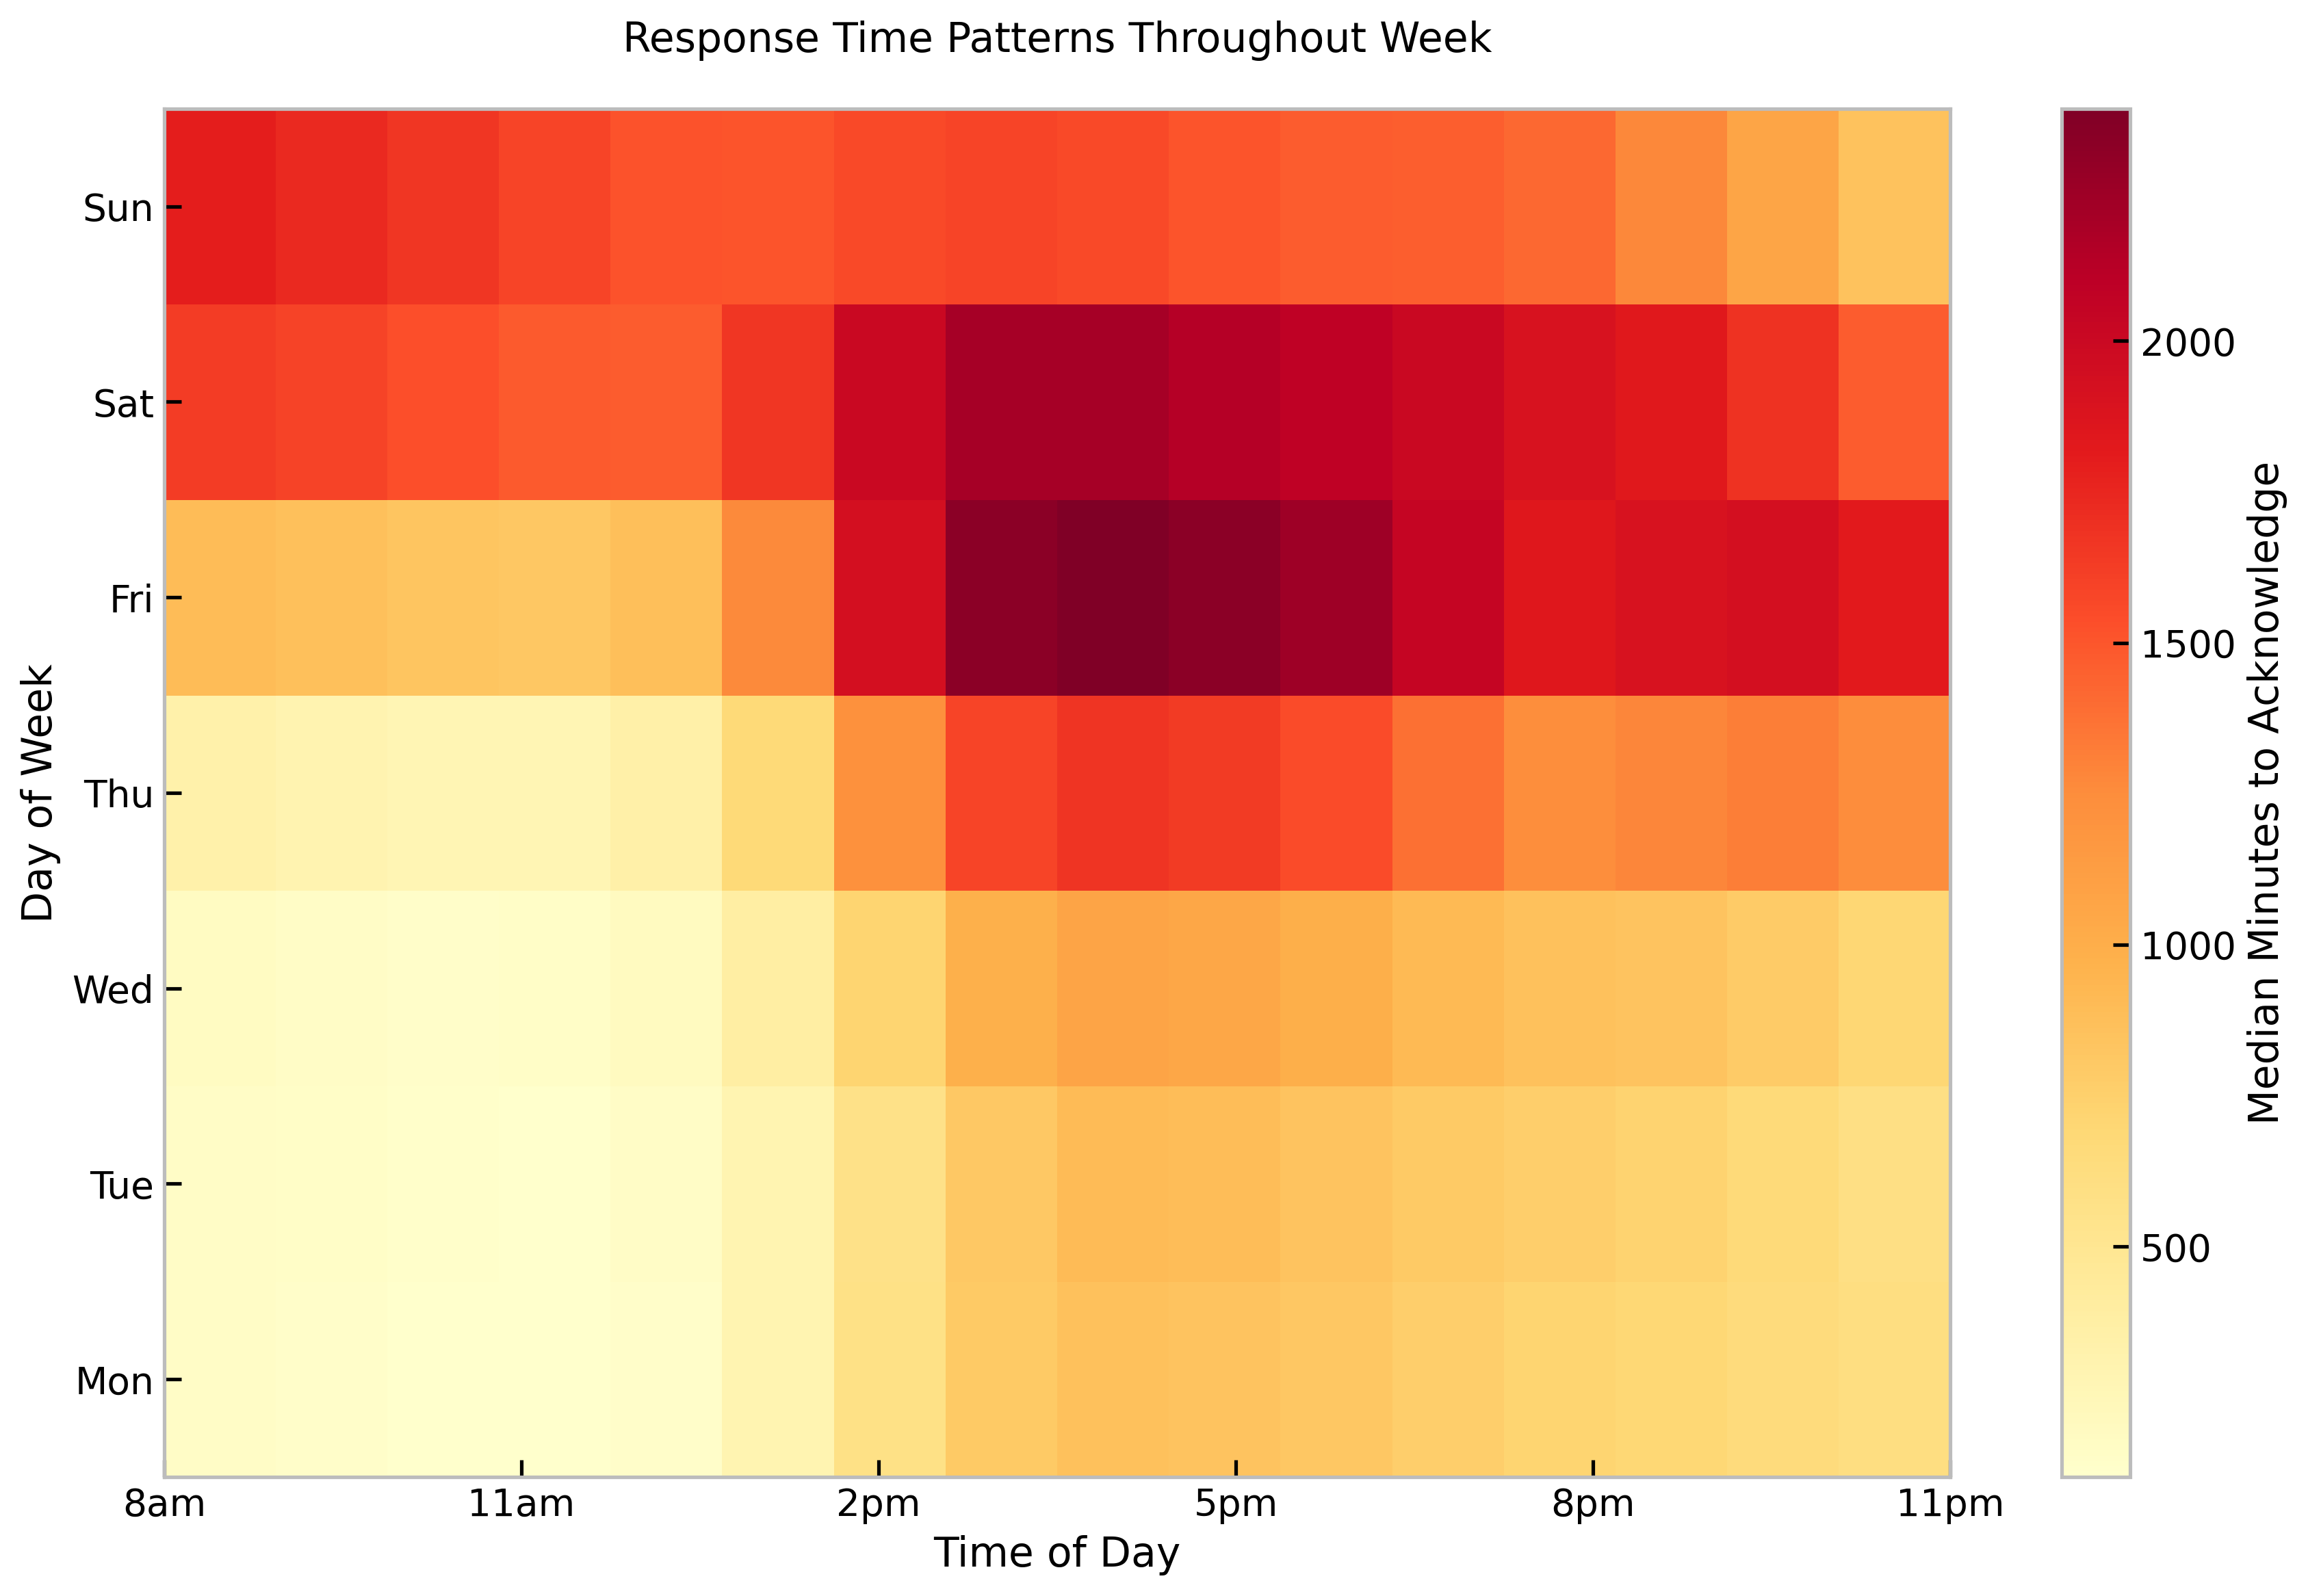
\includegraphics[width=\textwidth]{response_time_heatmap}
\caption{Response Time Patterns Throughout Week}
\label{fig:response_patterns}
\end{figure}

The heatmap visualization reveals several critical patterns in response times. Most notably, there is a significant slowdown in response times during weekends and Friday afternoons. The data shows:

\begin{itemize}
    \item Early weekday mornings (8am-11am) demonstrate the fastest response times
    \item Friday afternoons show a marked increase in response times, indicating potential end-of-week staffing challenges
    \item Weekend response times are consistently slower across all hours
    \item A clear "hot spot" of slower responses appears during Friday and Saturday afternoons
    \item Late evening hours (8pm-11pm) show gradually increasing response times
\end{itemize}

\section{Agency Performance Analysis}

\begin{figure}[H]
\centering
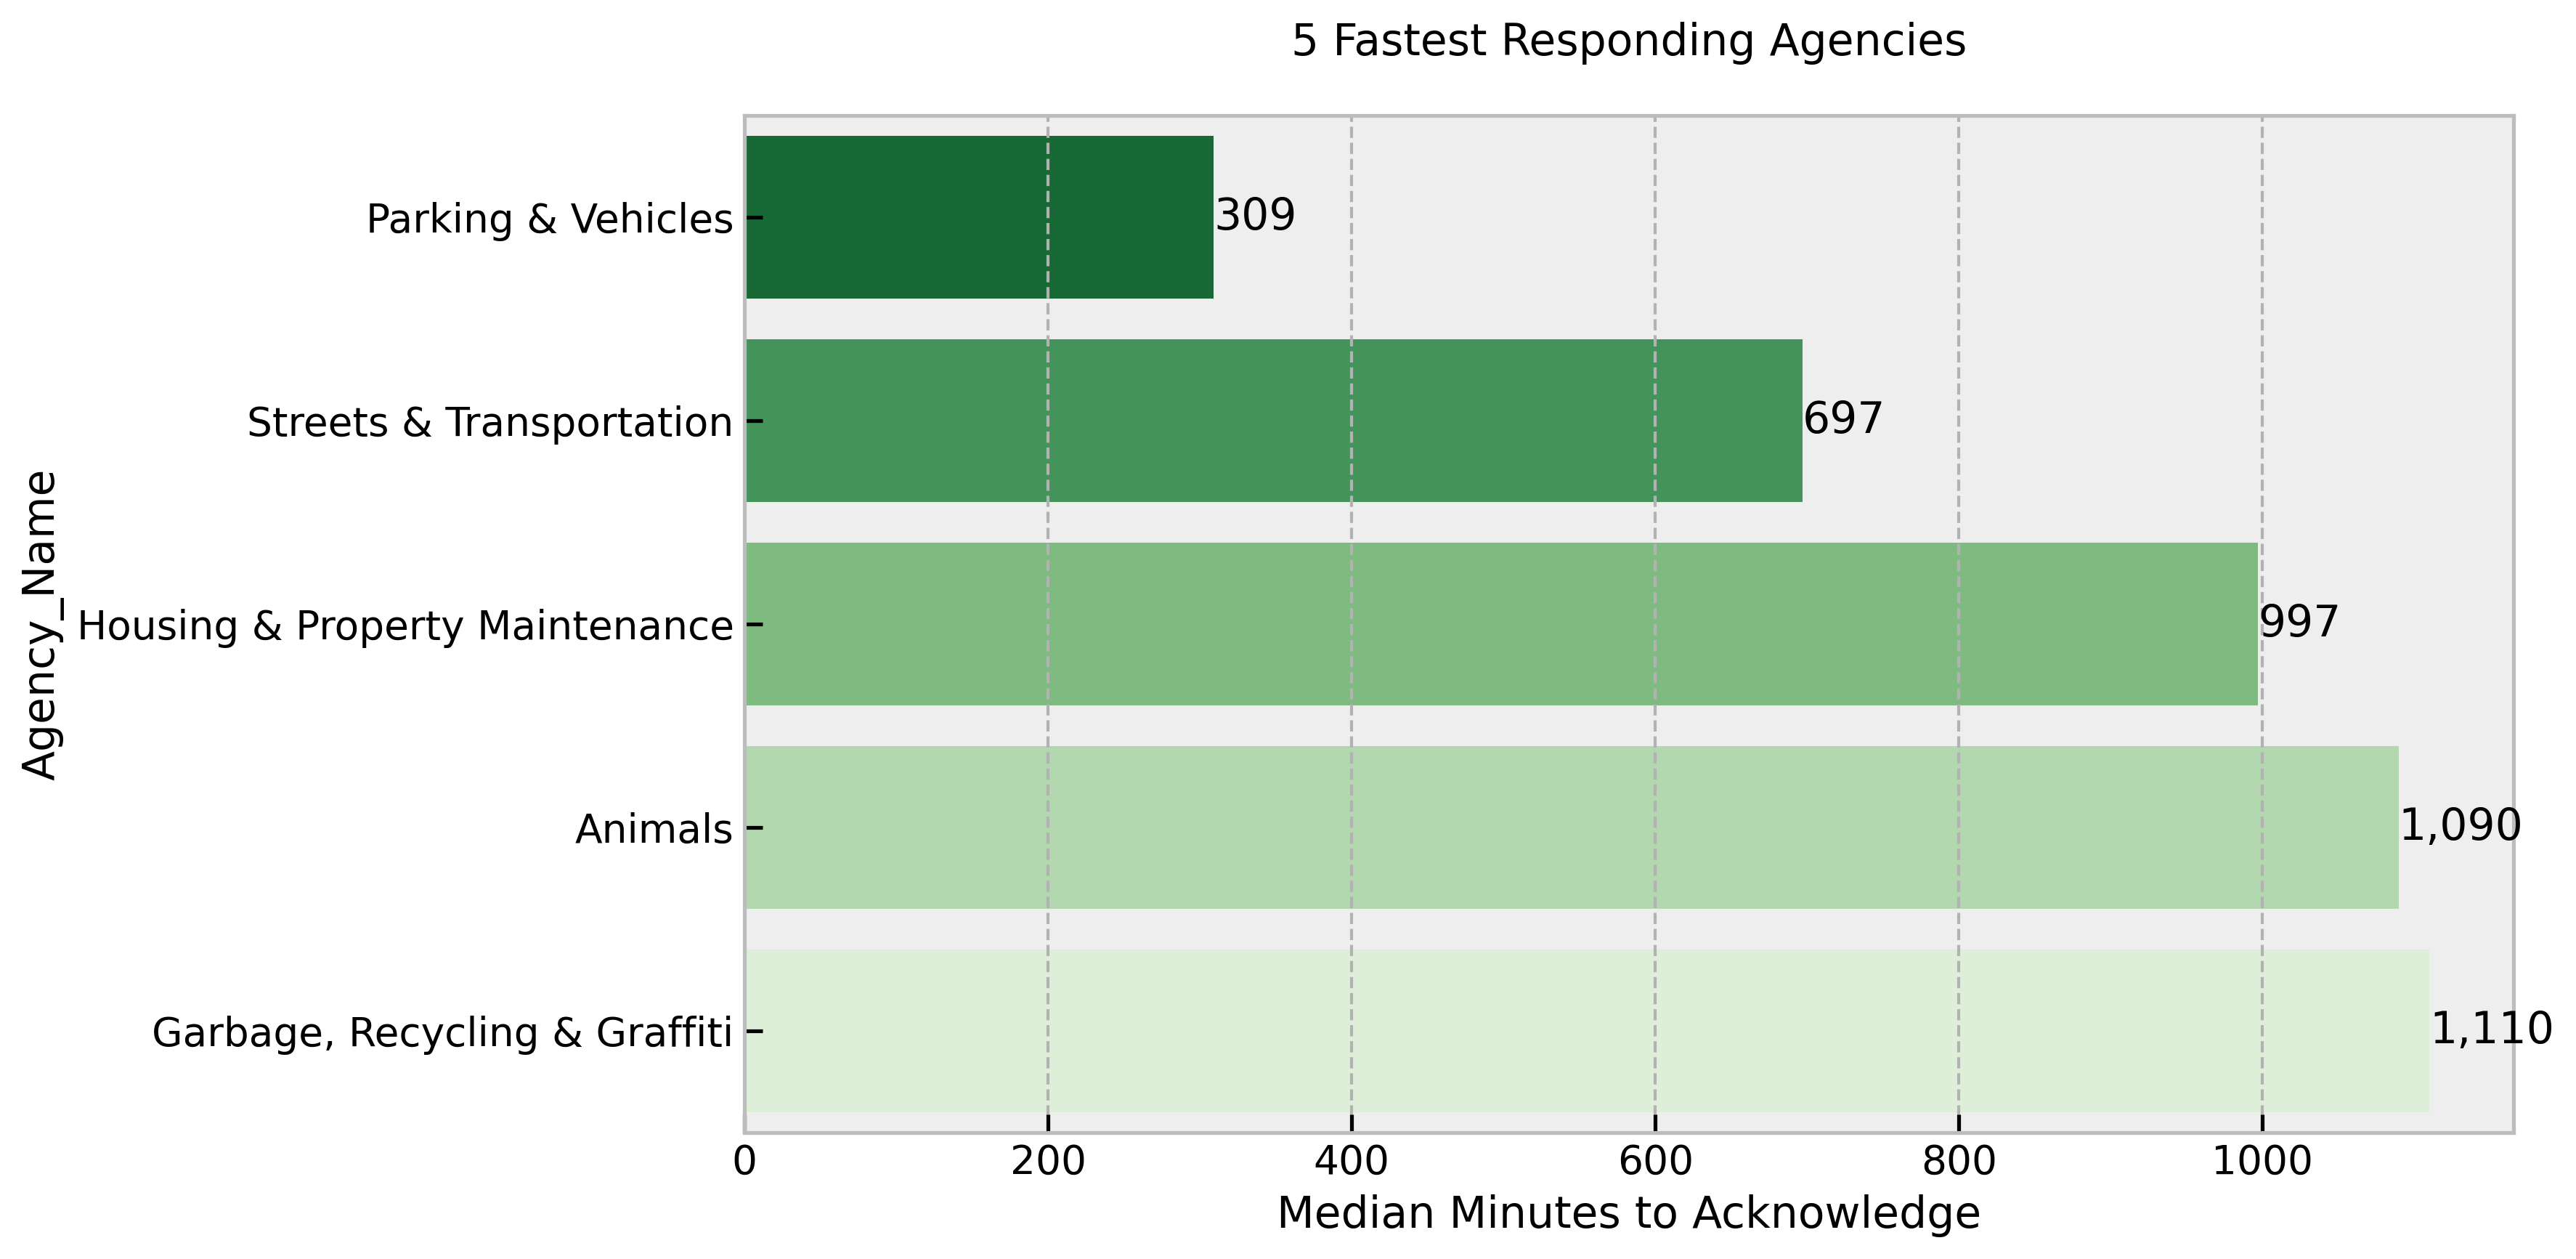
\includegraphics[width=0.8\textwidth]{fastest_agencies}
\caption{Top 5 Fastest Responding Agencies}
\label{fig:fast_agencies}
\end{figure}

\begin{figure}[H]
\centering
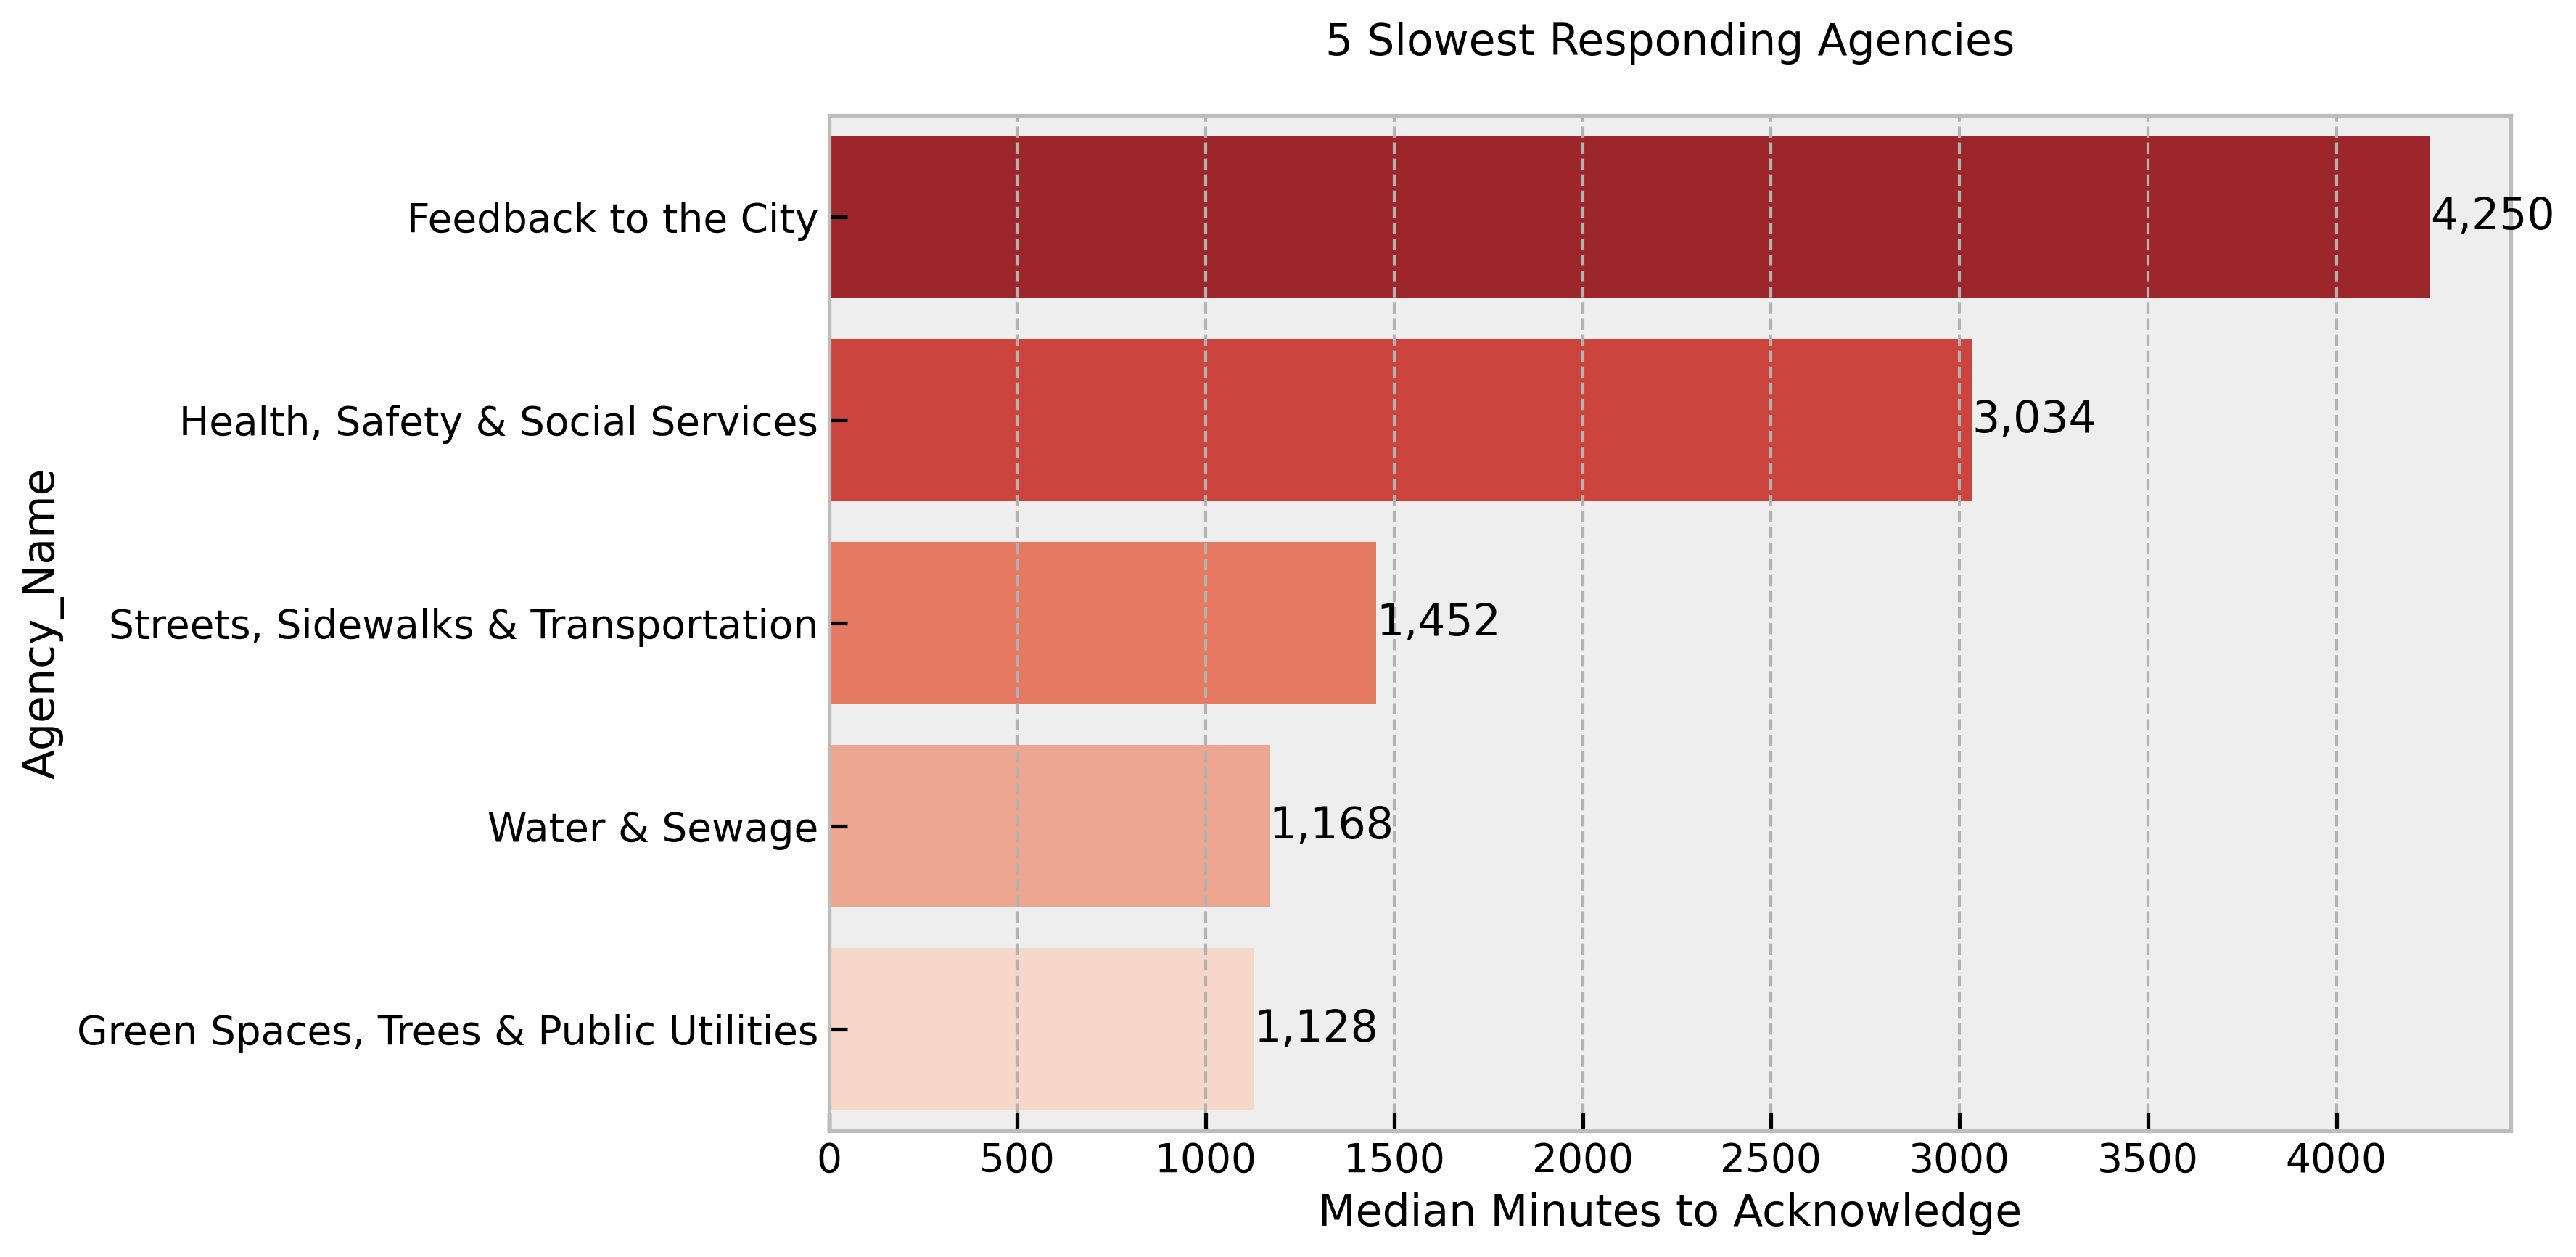
\includegraphics[width=0.8\textwidth]{slowest_agencies}
\caption{Top 5 Slowest Responding Agencies}
\label{fig:slow_agencies}
\end{figure}

\section{Assignee Performance Analysis}

\begin{figure}[H]
\centering
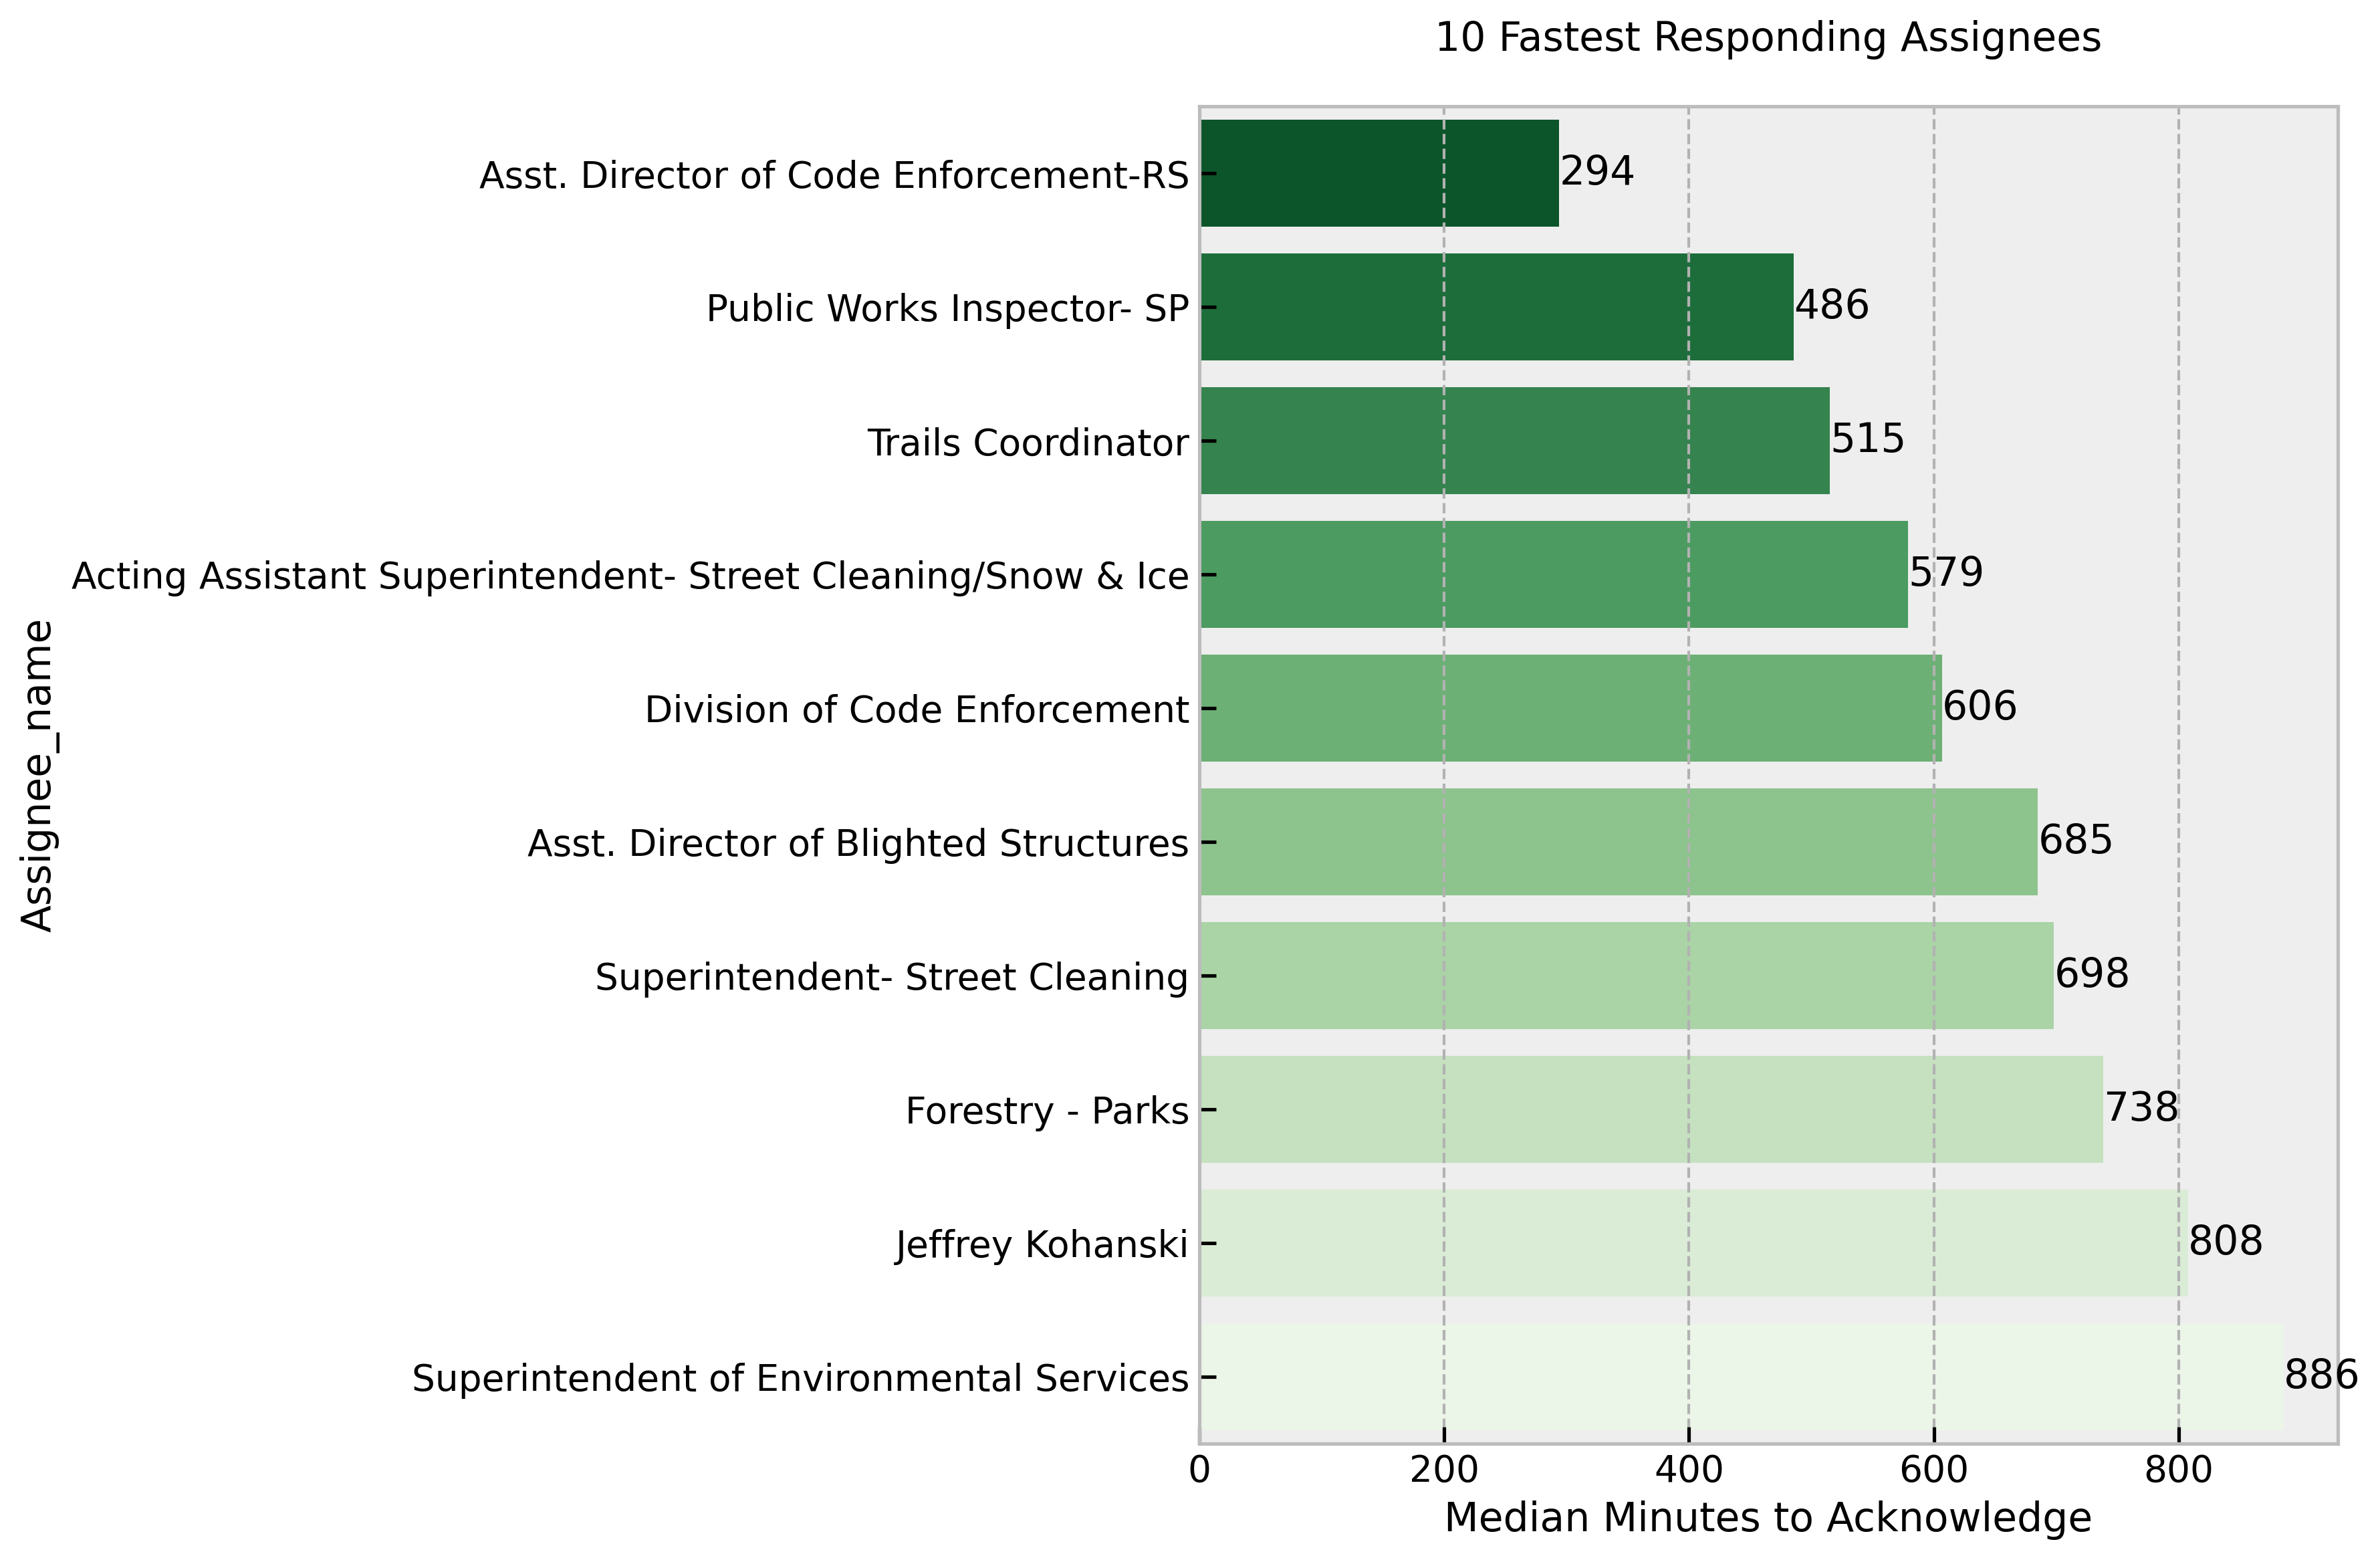
\includegraphics[width=0.8\textwidth]{fastest_assignees}
\caption{Top 10 Fastest Responding Assignees}
\label{fig:fast_assignees}
\end{figure}

\begin{figure}[H]
\centering
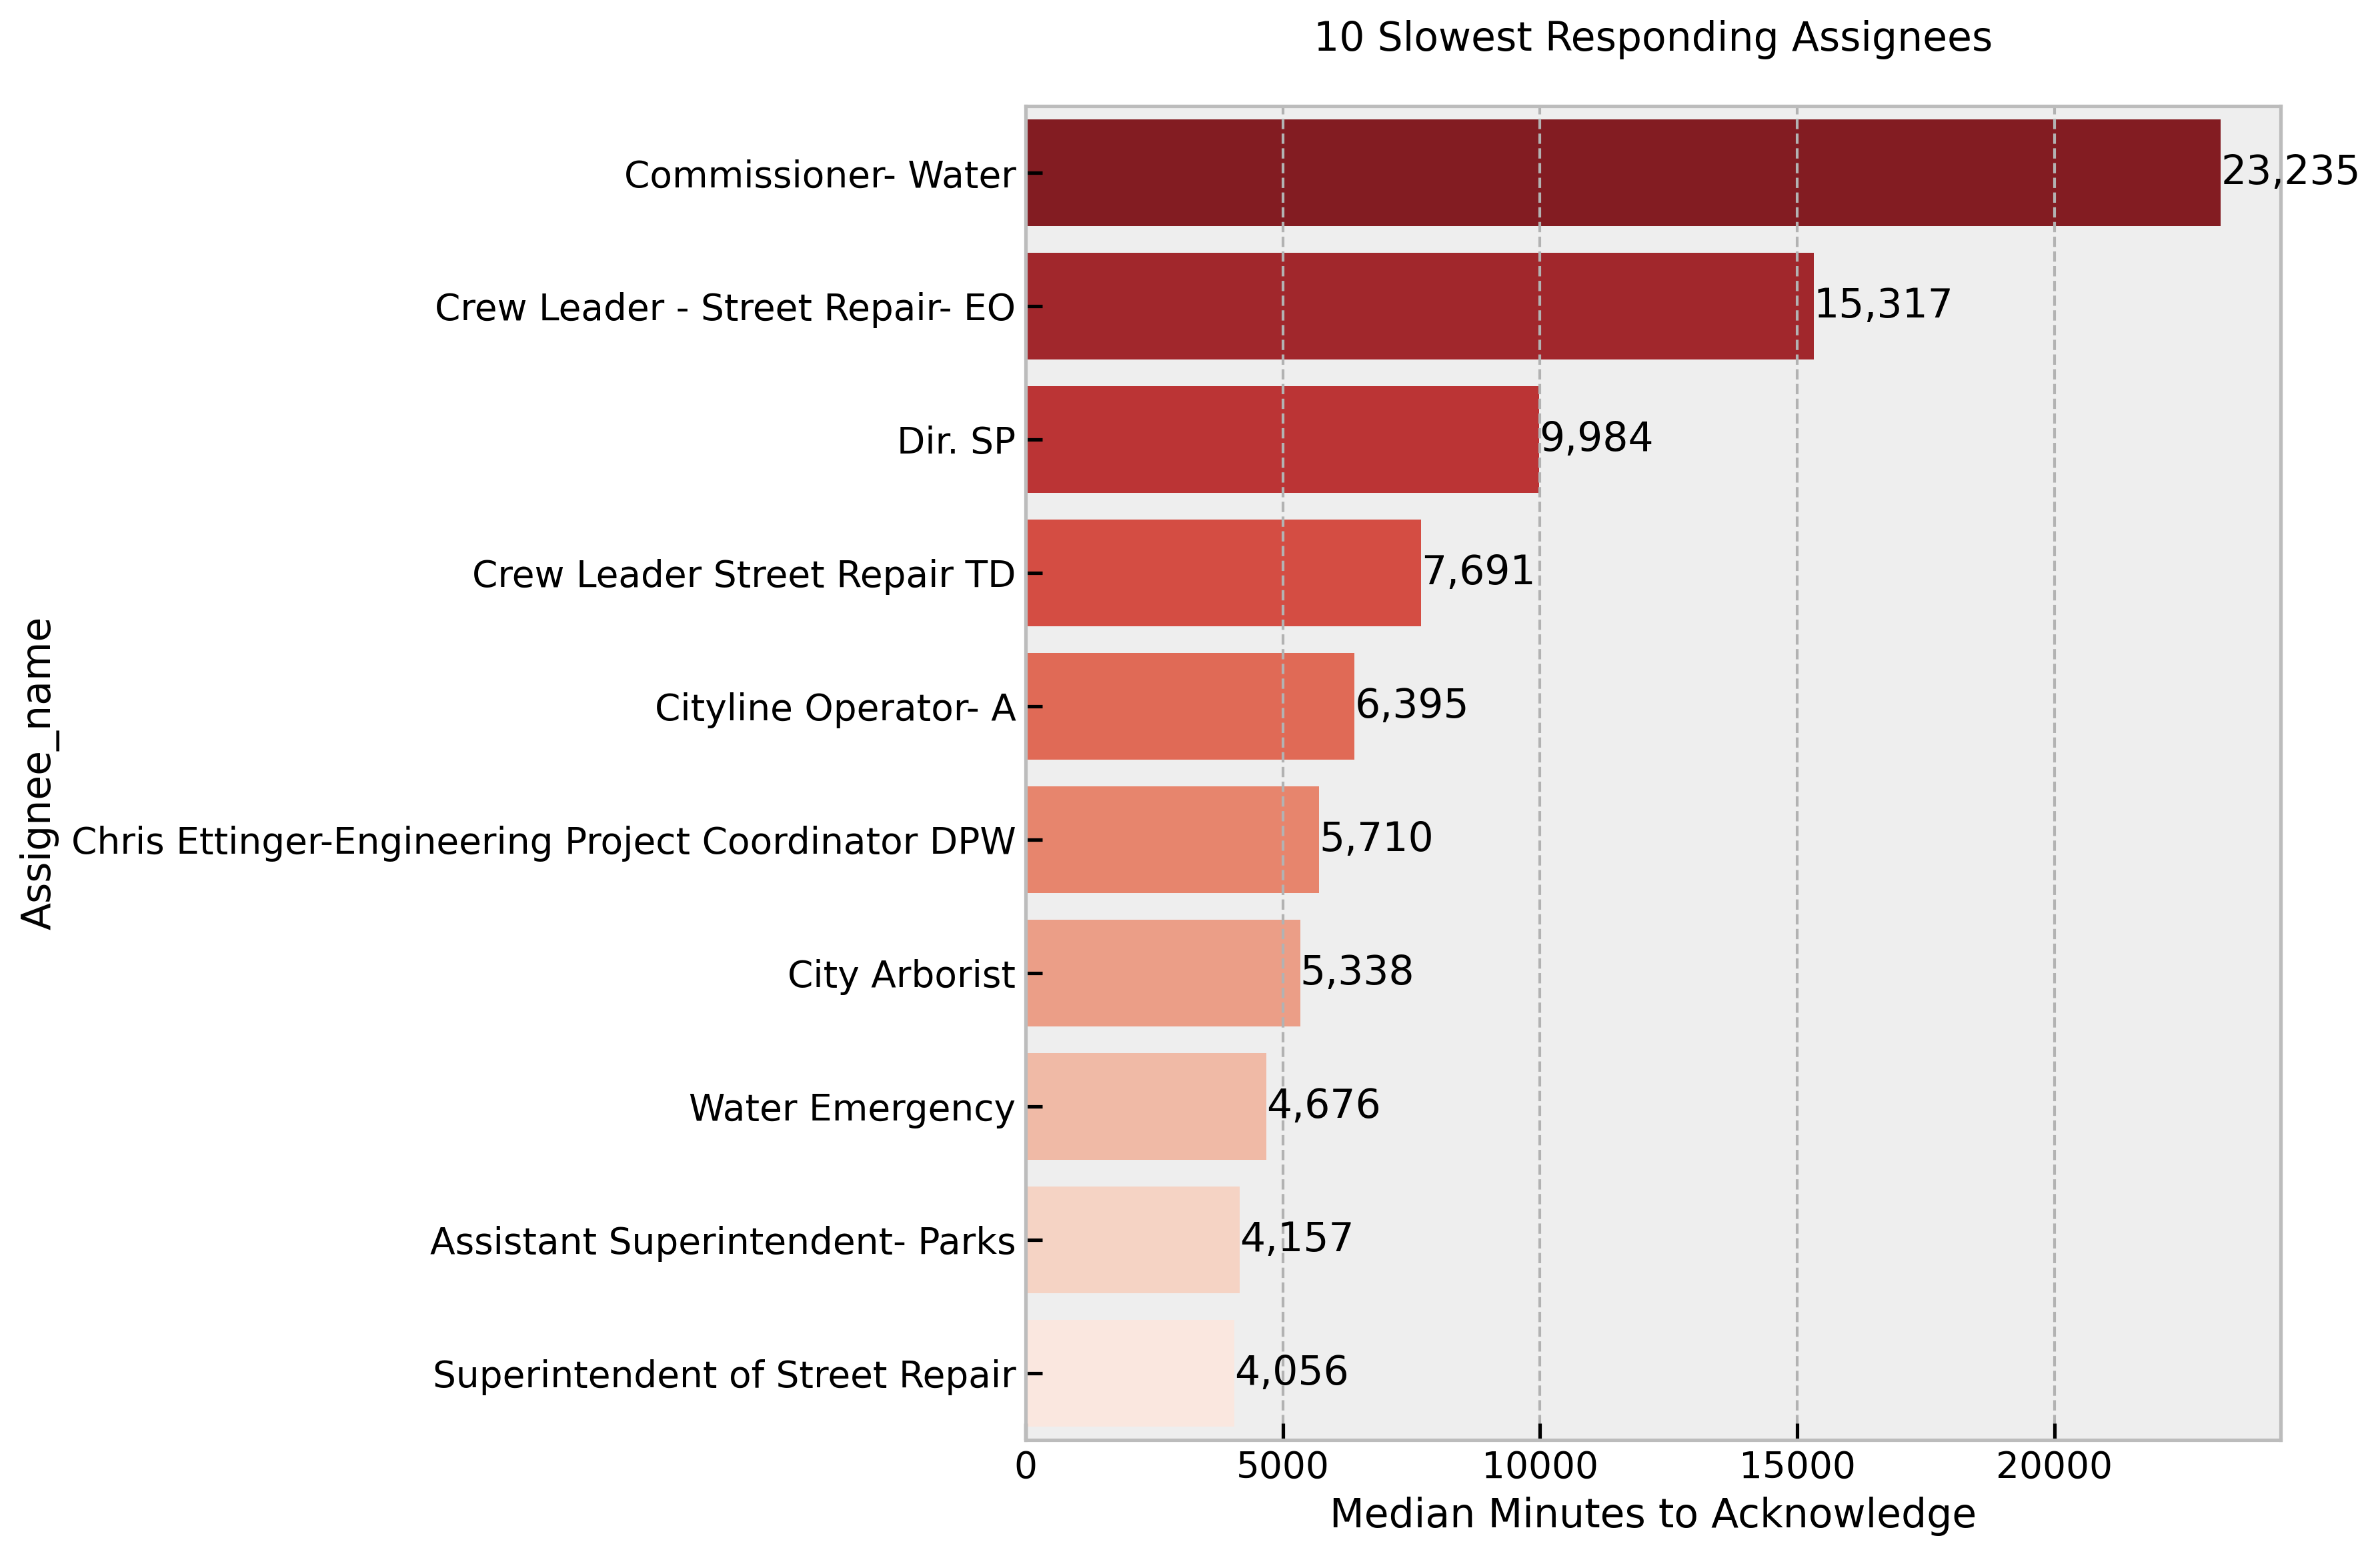
\includegraphics[width=0.8\textwidth]{slowest_assignees}
\caption{Top 10 Slowest Responding Assignees}
\label{fig:slow_assignees}
\end{figure}

\section{Category Performance Analysis}

\begin{figure}[H]
\centering
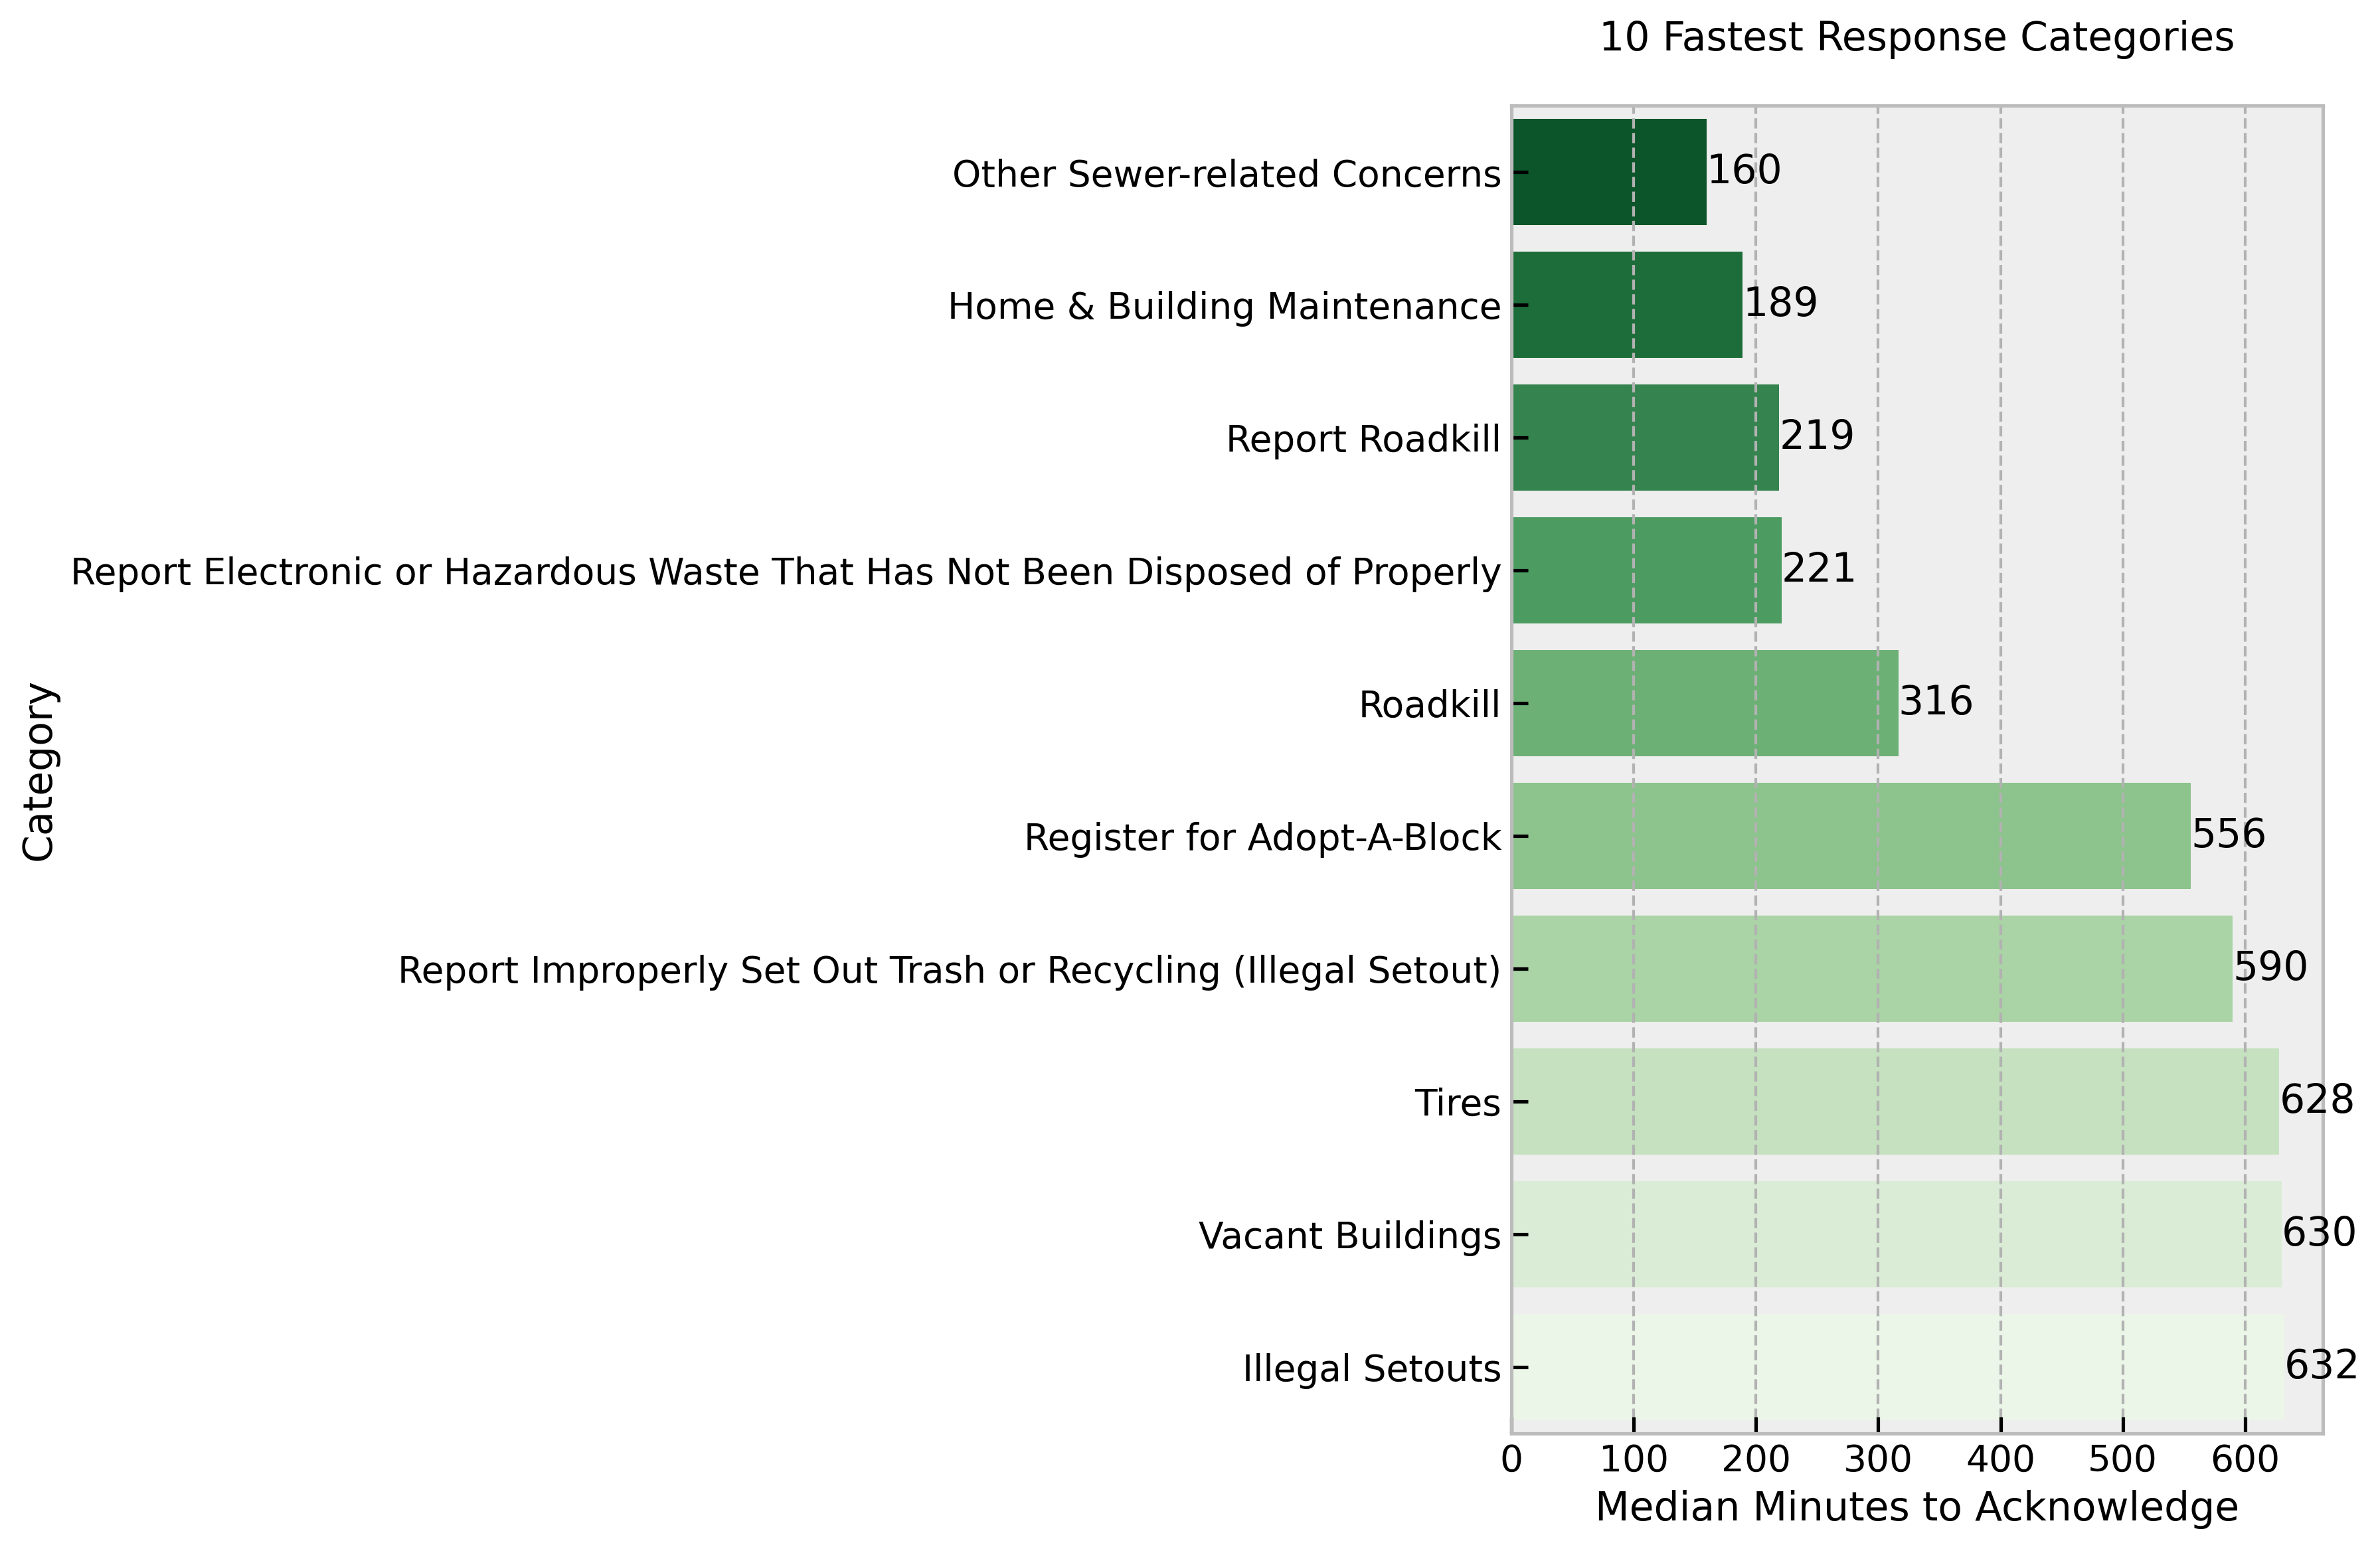
\includegraphics[width=0.8\textwidth]{fastest_categories}
\caption{Top 10 Fastest Acknowledged Categories}
\label{fig:fast_categories}
\end{figure}

\begin{figure}[H]
\centering
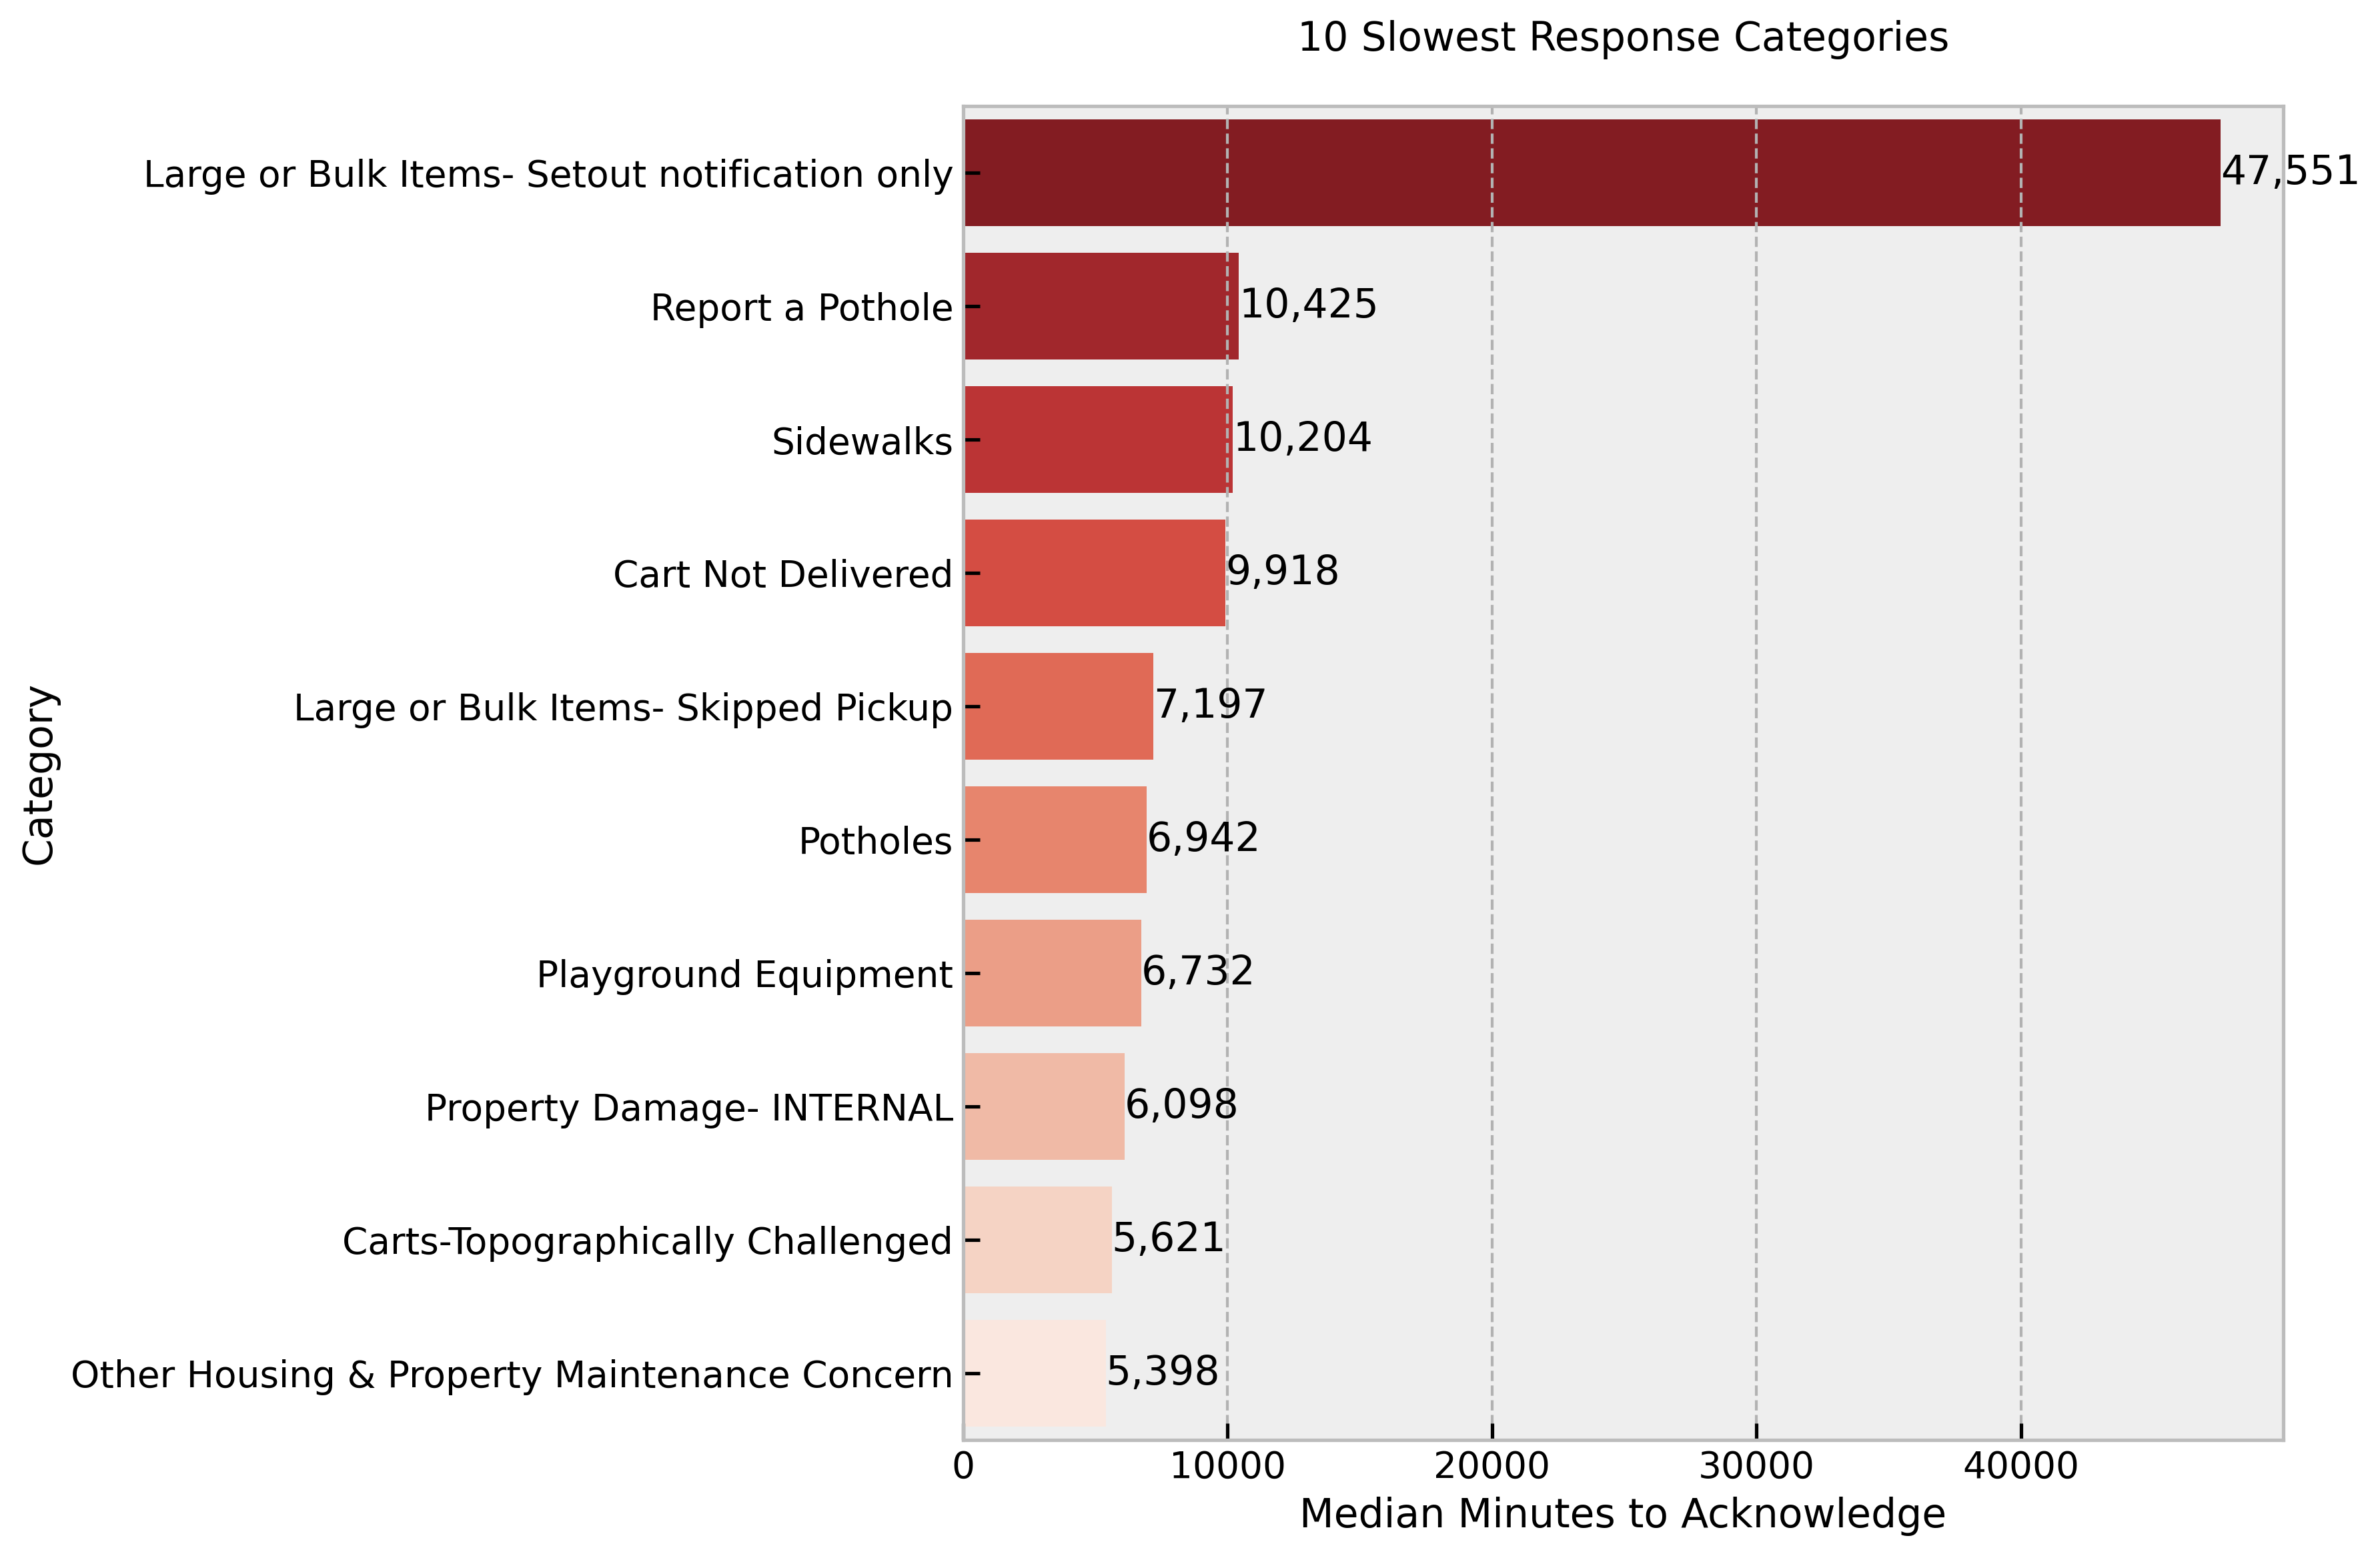
\includegraphics[width=0.8\textwidth]{slowest_categories}
\caption{Top 10 Slowest Acknowledged Categories}
\label{fig:slow_categories}
\end{figure}

\chapter{Compliance Rate Analysis}

\section{Overall Compliance Patterns}
The analysis reveals significant variations in compliance rates across different service categories, ranging from 18.3\% to 97.3\%. This wide range suggests systematic differences in either the difficulty of tasks, resource allocation, or process efficiency across different service types.

\section{Agency Compliance Analysis}
\subsection{Agency Performance Overview}

\begin{figure}[H]
\centering
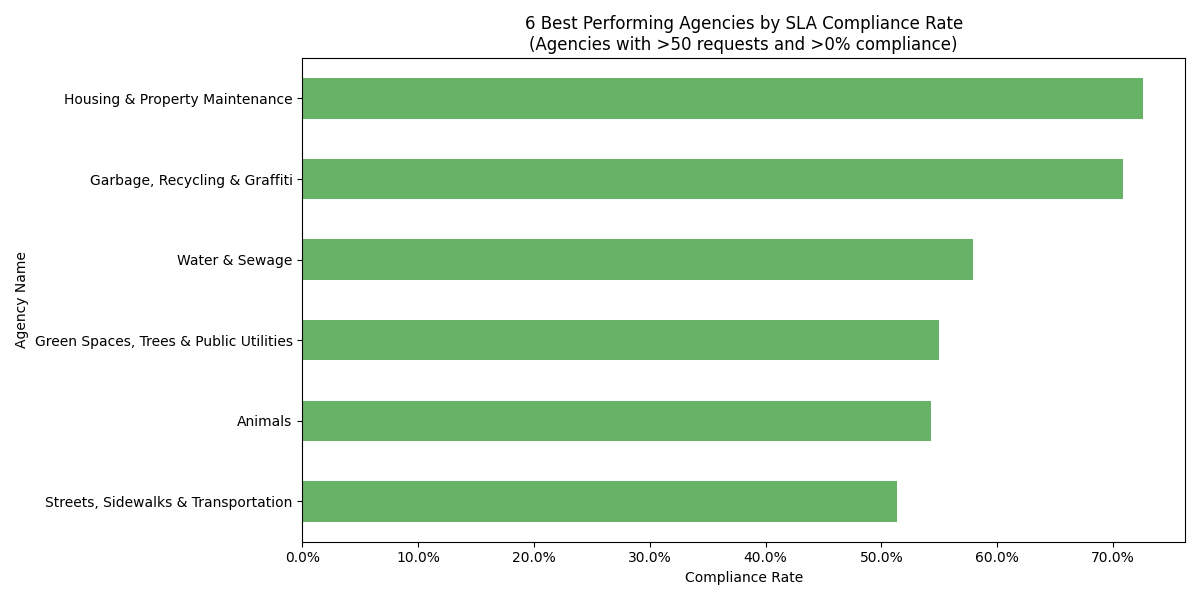
\includegraphics[width=0.8\textwidth]{best_performers_agency}
\caption{Best Performing Agencies by Compliance Rate}
\label{fig:best_agencies}
\end{figure}

\begin{figure}[H]
\centering
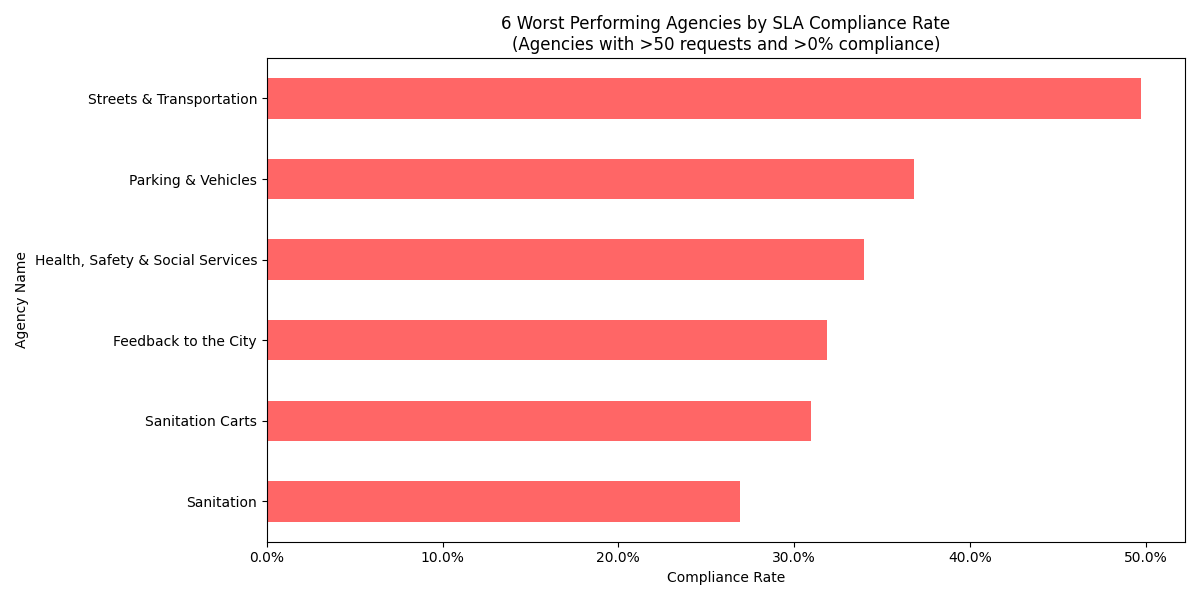
\includegraphics[width=0.8\textwidth]{worst_performers_agency}
\caption{Worst Performing Agencies by Compliance Rate}
\label{fig:worst_agencies}
\end{figure}

The analysis shows a stark contrast between high and low-performing agencies, with compliance rates ranging from 72.6\% to 26.9\%. Housing \& Property Maintenance leads with the highest compliance rate while handling a substantial volume of requests.

\section{Assignee Compliance Analysis}

\begin{figure}[H]
\centering
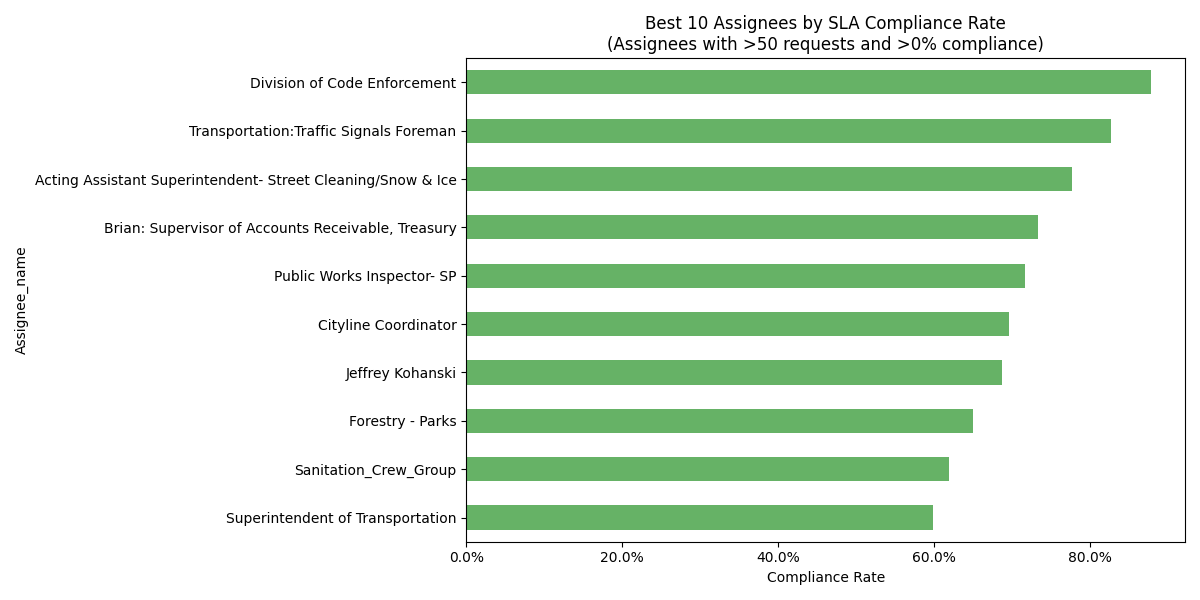
\includegraphics[width=0.8\textwidth]{best_performers_assignee}
\caption{Best Performing Assignees by Compliance Rate}
\label{fig:best_assignees}
\end{figure}

\begin{figure}[H]
\centering
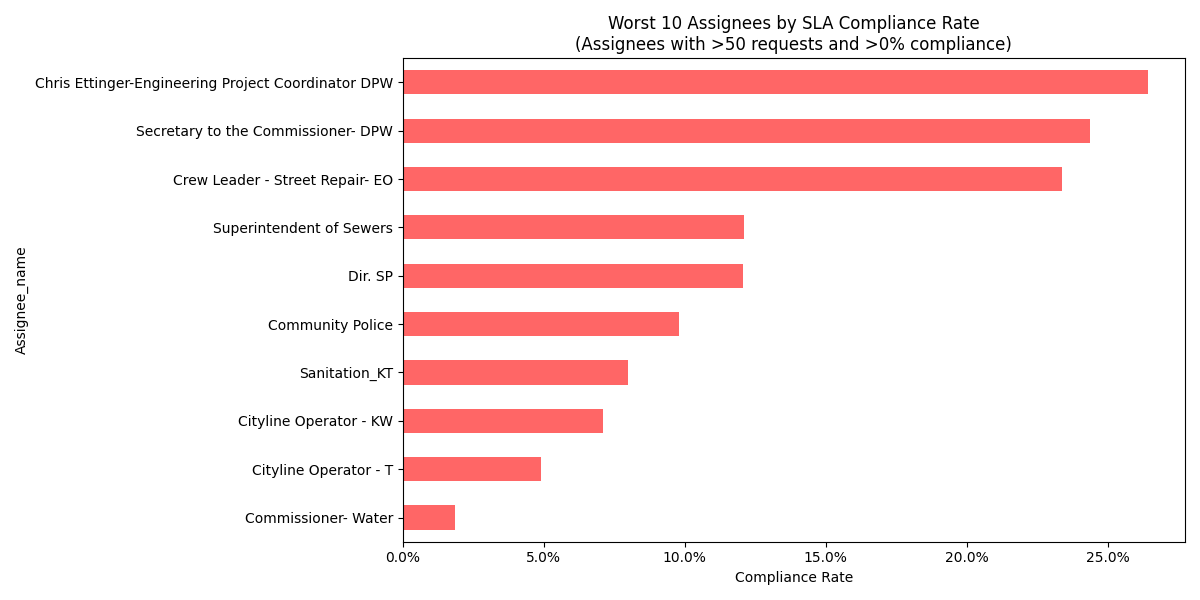
\includegraphics[width=0.8\textwidth]{worst_performers_assignee}
\caption{Worst Performing Assignees by Compliance Rate}
\label{fig:worst_assignees}
\end{figure}

Individual assignee performance shows significant variation, with the Division of Code Enforcement achieving the highest compliance rate at 87.8\% while handling a substantial volume of 7,839 requests.

\section{Category Performance Analysis}

\begin{figure}[H]
\centering
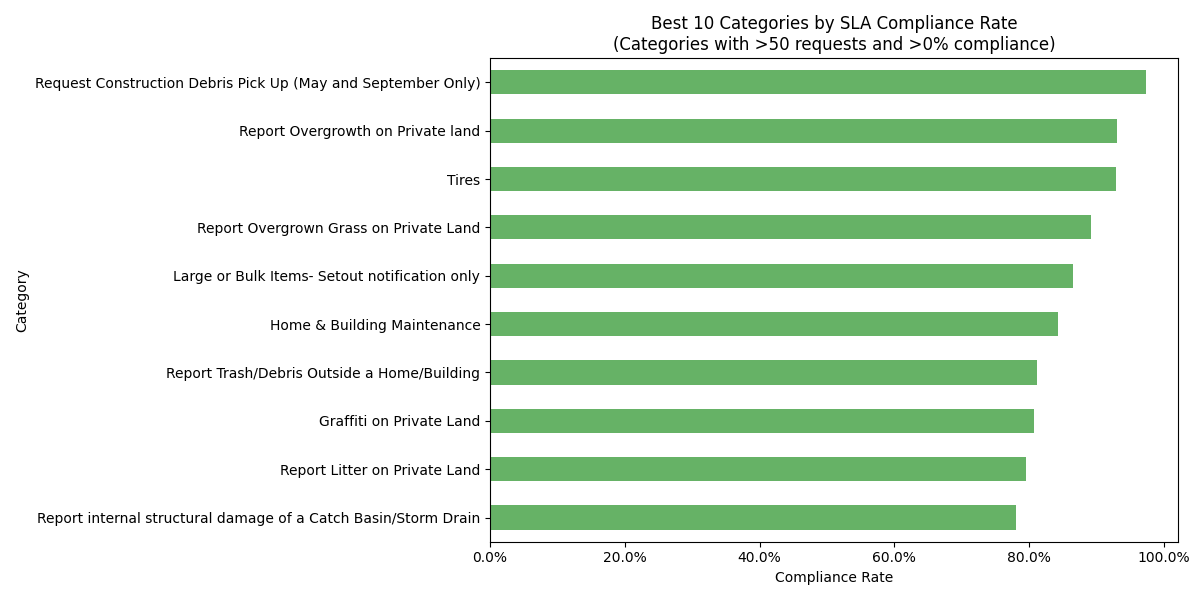
\includegraphics[width=0.8\textwidth]{best_performers_categories}
\caption{Best Performing Service Categories by Compliance Rate}
\label{fig:best_categories}
\end{figure}

\begin{figure}[H]
\centering
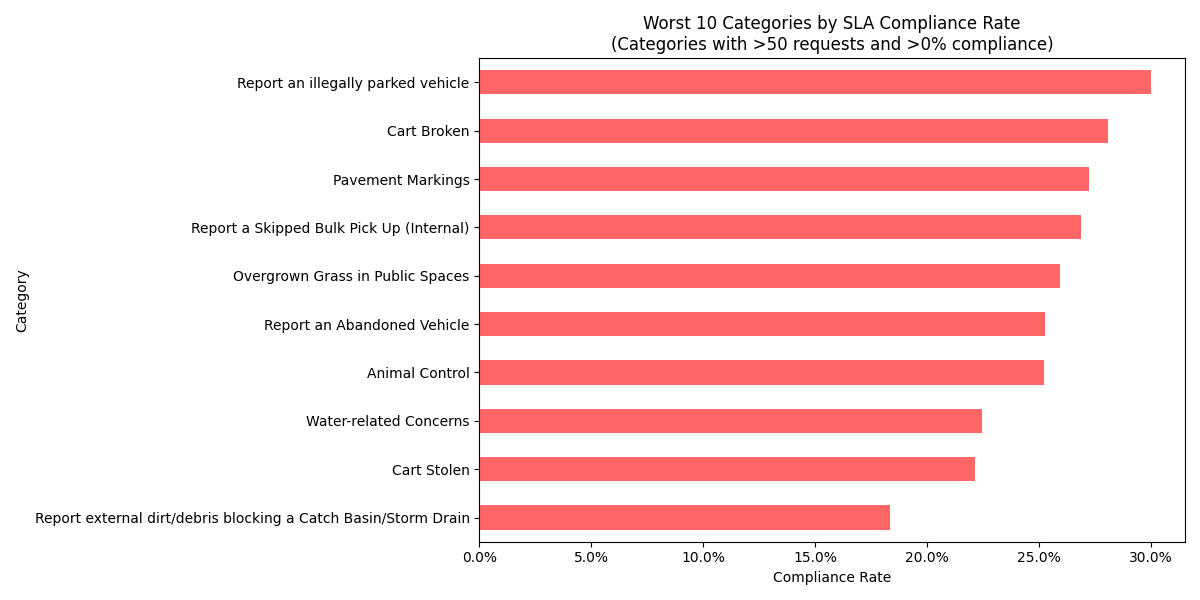
\includegraphics[width=0.8\textwidth]{worst_performers_categories}
\caption{Worst Performing Service Categories by Compliance Rate}
\label{fig:worst_categories}
\end{figure}

\section{Cross-Dimensional Analysis}
The data reveals several key patterns across agencies, assignees, and categories:

\begin{itemize}
    \item Property-related services generally show higher compliance rates
    \item Emergency or time-sensitive services often have lower compliance rates
    \item High-volume categories tend to have more standardized performance
    \item Specialized services show greater variation in compliance
\end{itemize}

These patterns suggest that service complexity, resource allocation, and process standardization all play crucial roles in determining compliance rates.
\chapter{Recommendations and Insights}

\section{Key Findings}
\begin{enumerate}
    \item Historical performance metrics are the strongest predictors of future compliance
    \item Temporal factors (day of week, year) significantly impact service delivery
    \item Public engagement (followers) influences request completion
    \item Significant disparities exist in performance across agencies and categories
    \item Weekend and Friday afternoon response times show consistent delays
\end{enumerate}

\section{Actionable Recommendations}
\begin{enumerate}
    \item Implement targeted training for low-performing assignees
    \item Review and optimize processes for categories with compliance rates below 30\%
    \item Develop standardized response protocols for high-volume request types
    \item Consider workload reallocation based on historical performance metrics
    \item Strengthen weekend and Friday afternoon staffing levels
\end{enumerate}

\end{document}